\documentclass{article}
\usepackage[margin=1in]{geometry}
\usepackage{amsmath}
\usepackage{ctex}
\usepackage{siunitx}
\usepackage{multirow}
\usepackage{bigstrut}
\usepackage{graphicx}
\usepackage{hyperref}
\title{整流滤波实验报告}
\author{姓名:宋建宏\,\, 学号:PB21020677\,\, 班级:203院22级5班\\ 日期:2023年4月23日}
\date{}

\begin{document}
\maketitle
\section*{实验目的}
了解整流滤波电路的基本原理,学习电路实验操作。

\section*{实验原理}

整流就是将交变电流转换成直流电流的一种方法,在实验中我们采用二极管来完成整流。而滤波是把大脉动直流电处理成平滑的脉动小的直流电。

\subsection*{整流原理}
在本实验中我们选择使用二极管来达到整流目的,在实验中将尝试半波整流和全波整流。

半波整流原理较简单,就是通过一个二极管将反向的电流“截断”,如下图所示,反向的电流“消失”了。
而全波整流通过一个“电桥”使得两个方向的电流都能够转变为同向。

\begin{figure}[htbp]
    \centering
    \begin{minipage}[t]{0.48\textwidth}
        \centering
        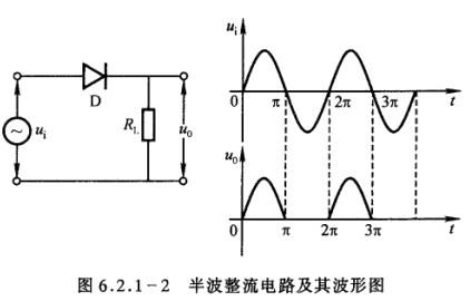
\includegraphics[scale=0.8]{figures/bbzldl.png}

    \end{minipage}
    \begin{minipage}[t]{0.48\textwidth}
        \centering
        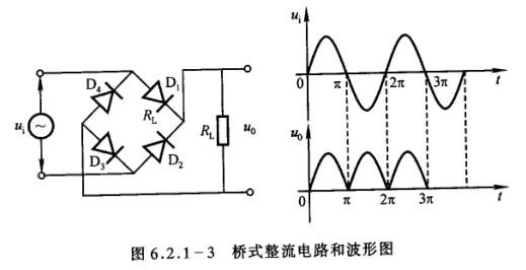
\includegraphics[scale=0.8]{figures/qbzldl.png}
    \end{minipage}
\end{figure}


\subsection*{滤波原理}
\subsubsection*{单电容滤波}
在交流电变化一个周期的过程中,由于二极管的单向导通性,使得电容器被充、放电。 如此周而复始,
形成了周期性的电容器充电放电过程。由于电容器的电压不能突变,故在这一小段时间内,它可被看成一个
反电动势。 由电容两端的电压不能突变的特点, 可达到输出波形趋于平滑的目的。

\subsubsection*{$\pi$型RC滤波}
前述电容滤波的输出波形脉动仍较大,尤其是负载电阻$R_L$较小时。除非将电容容量增加(实际应用时难
于实现)。在这种情况下,要想减少脉动可利用多级滤波方法,此时再加一级RC低通滤波电路,如图所示,
这种电路也称$\pi$型RC滤波电路,这种方法使得输出电压更平滑(但输出电压平均值要减少)。

\begin{figure}[htbp]
    \centering
    \begin{minipage}[t]{0.48\textwidth}
        \centering
        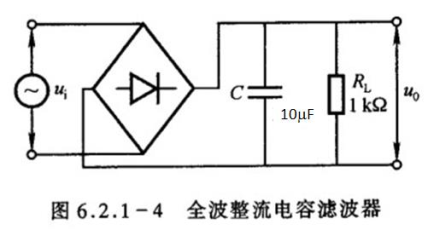
\includegraphics[scale=0.9]{figures/lbdl.png}

    \end{minipage}
    \begin{minipage}[t]{0.48\textwidth}
        \centering
        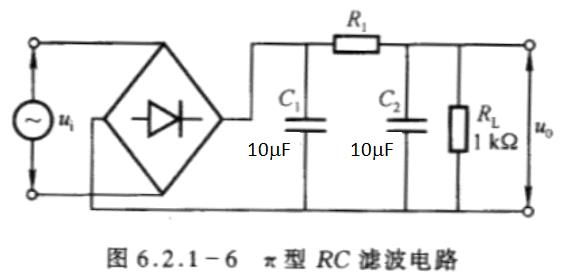
\includegraphics[scale=0.8]{figures/pilbdl.png}
    \end{minipage}
\end{figure}

\subsection*{波纹系数}
直流稳压电源一般是由交流电源经过整流滤波稳压等环节而形成的,直流稳定量中不可避免地带
有一些交流成分,这种叠加在直流稳定量上的交流分量就称之为纹波。一般可以用交流成分的有效值来表示纹波
绝对强度的大小。 纹波系数是指负载上交流电压的有效值与直流电压之比
\begin{equation*}
    \text{波纹系数}K_u=\frac{\text{交流电压有效值}}{\text{直流电压}}\times 100\%
\end{equation*}
是表征直流电源品质的一个重要参数。除了与整流滤波电路品质有关之外,与外电路负载关系也很大。

\section*{实验仪器}
信号发生器,示波器,数字电压表,面包板,二极管,电容,电阻,导线若干。

\section*{测量记录}
\subsection*{基础实验}滤波电路电压和整流滤波电路波形如下。
\begin{figure*}[h]
    \centering
    \begin{minipage}[t]{0.48\textwidth}
        \centering
        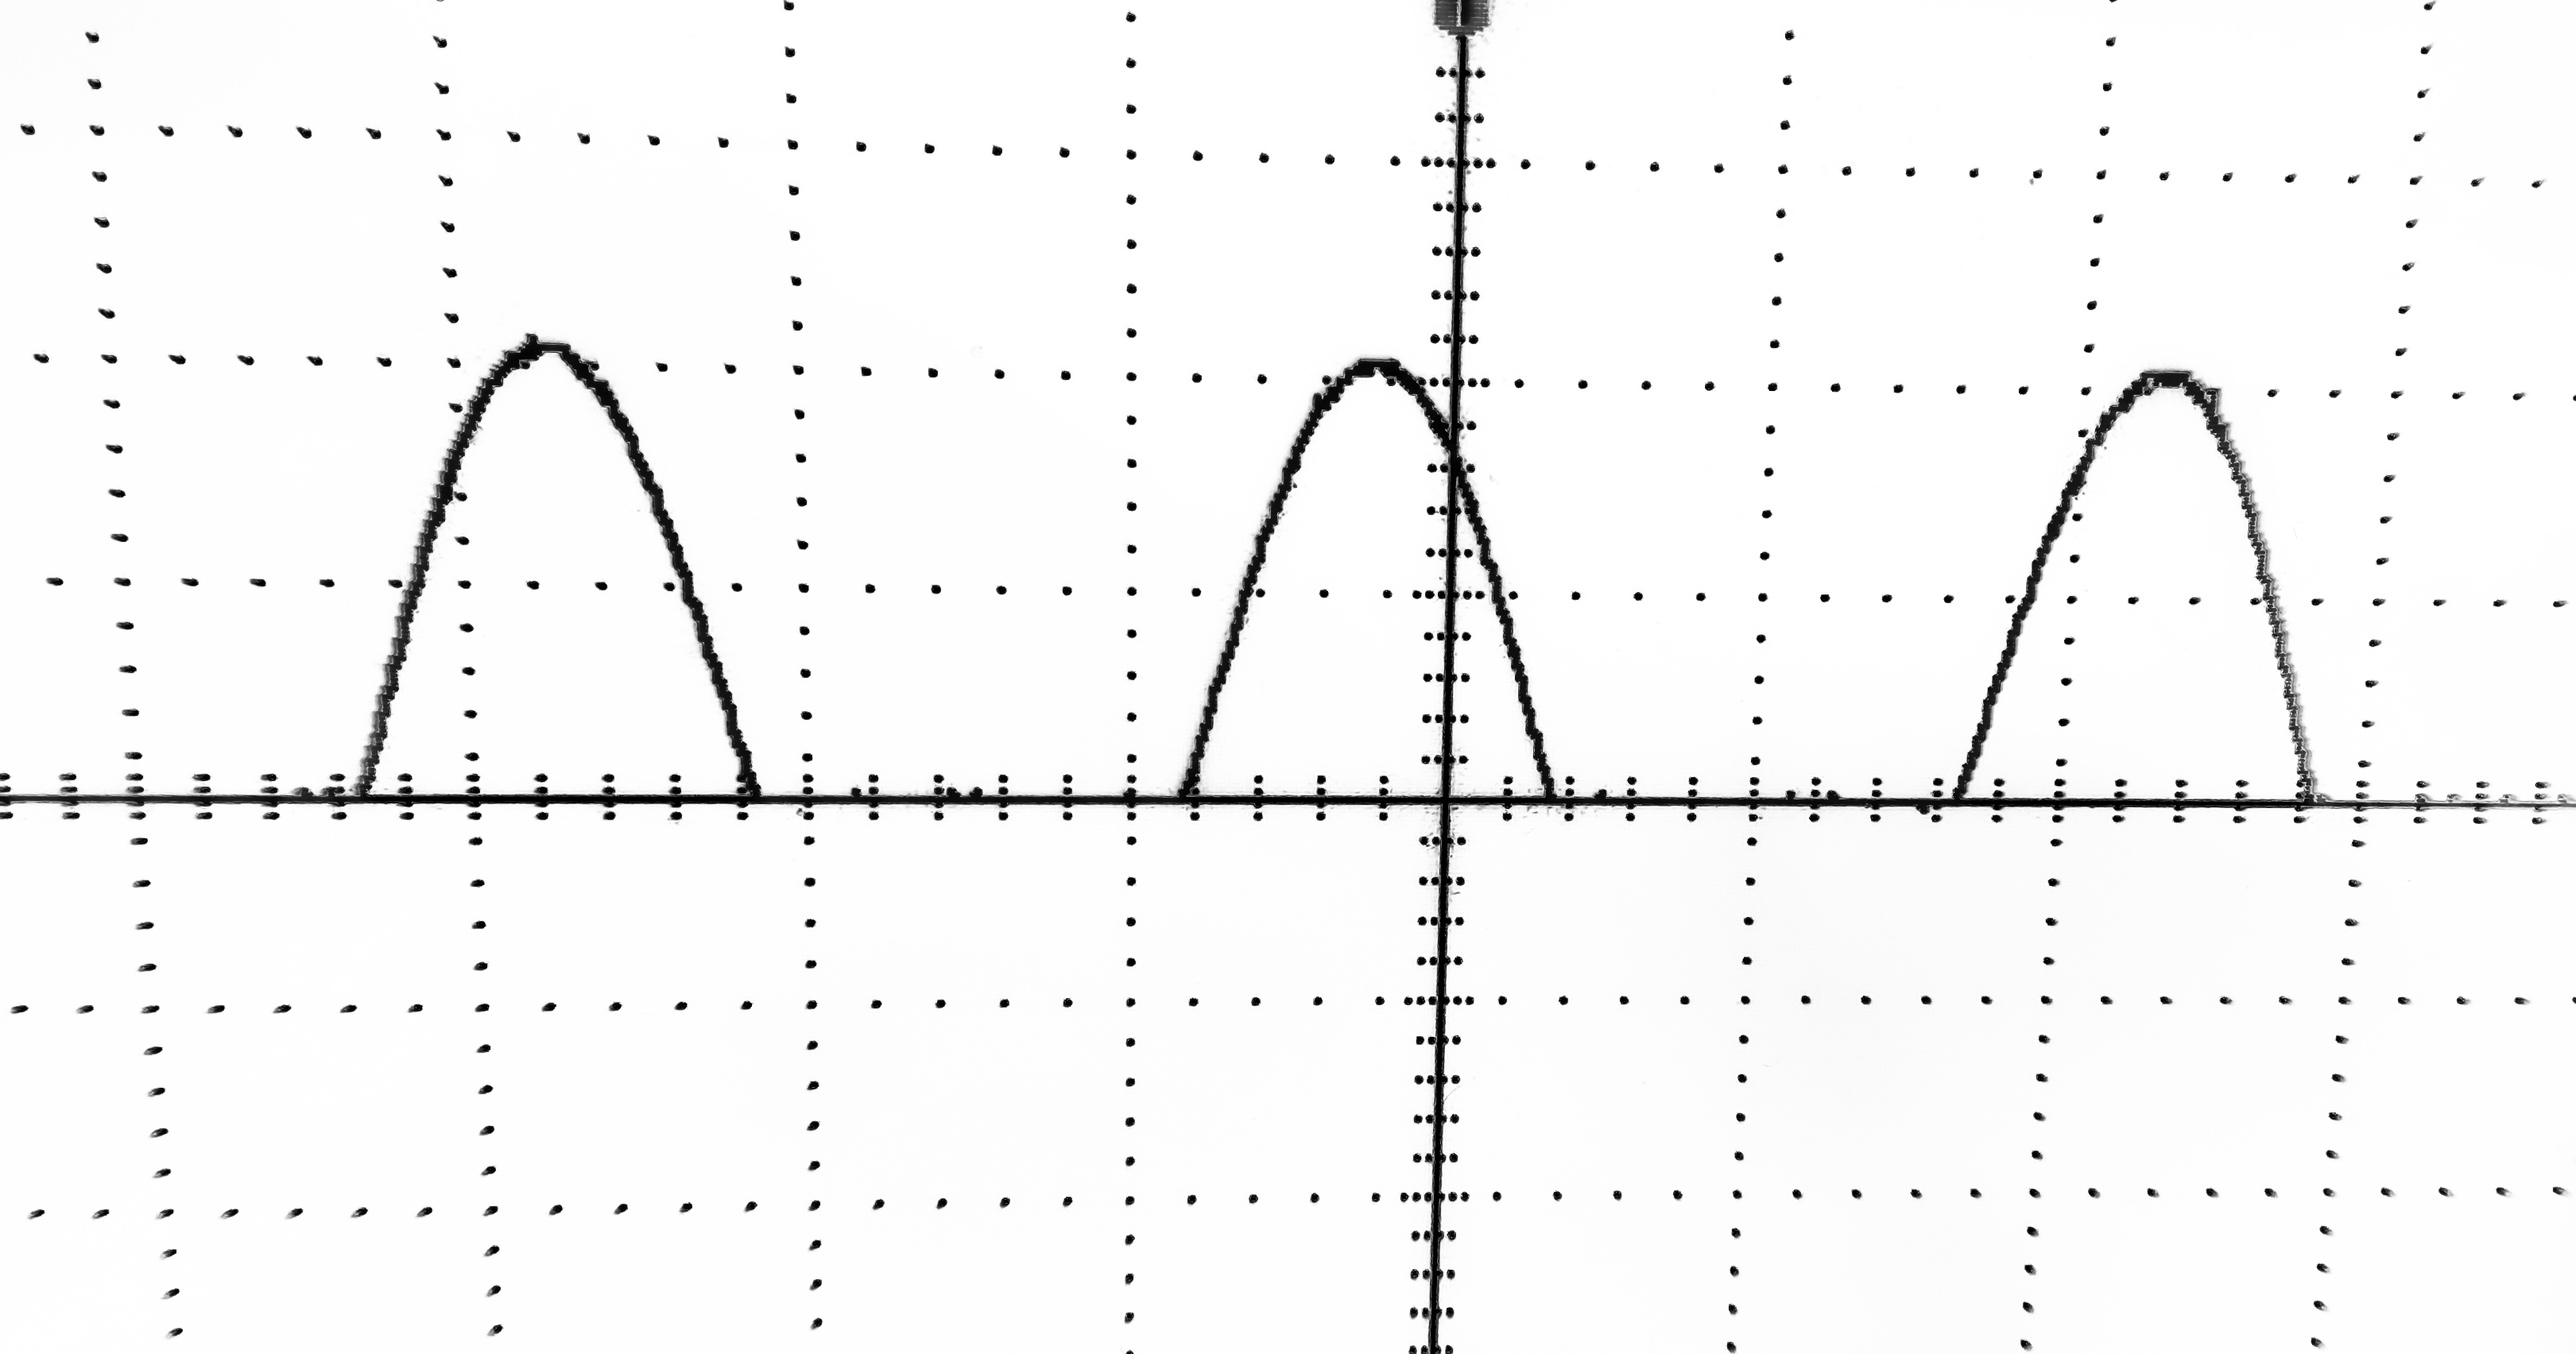
\includegraphics[scale=0.065]{figures/bbzl.png}
        \caption{半波整流波形图}
    \end{minipage}
    \begin{minipage}[t]{0.48\textwidth}
        \centering
        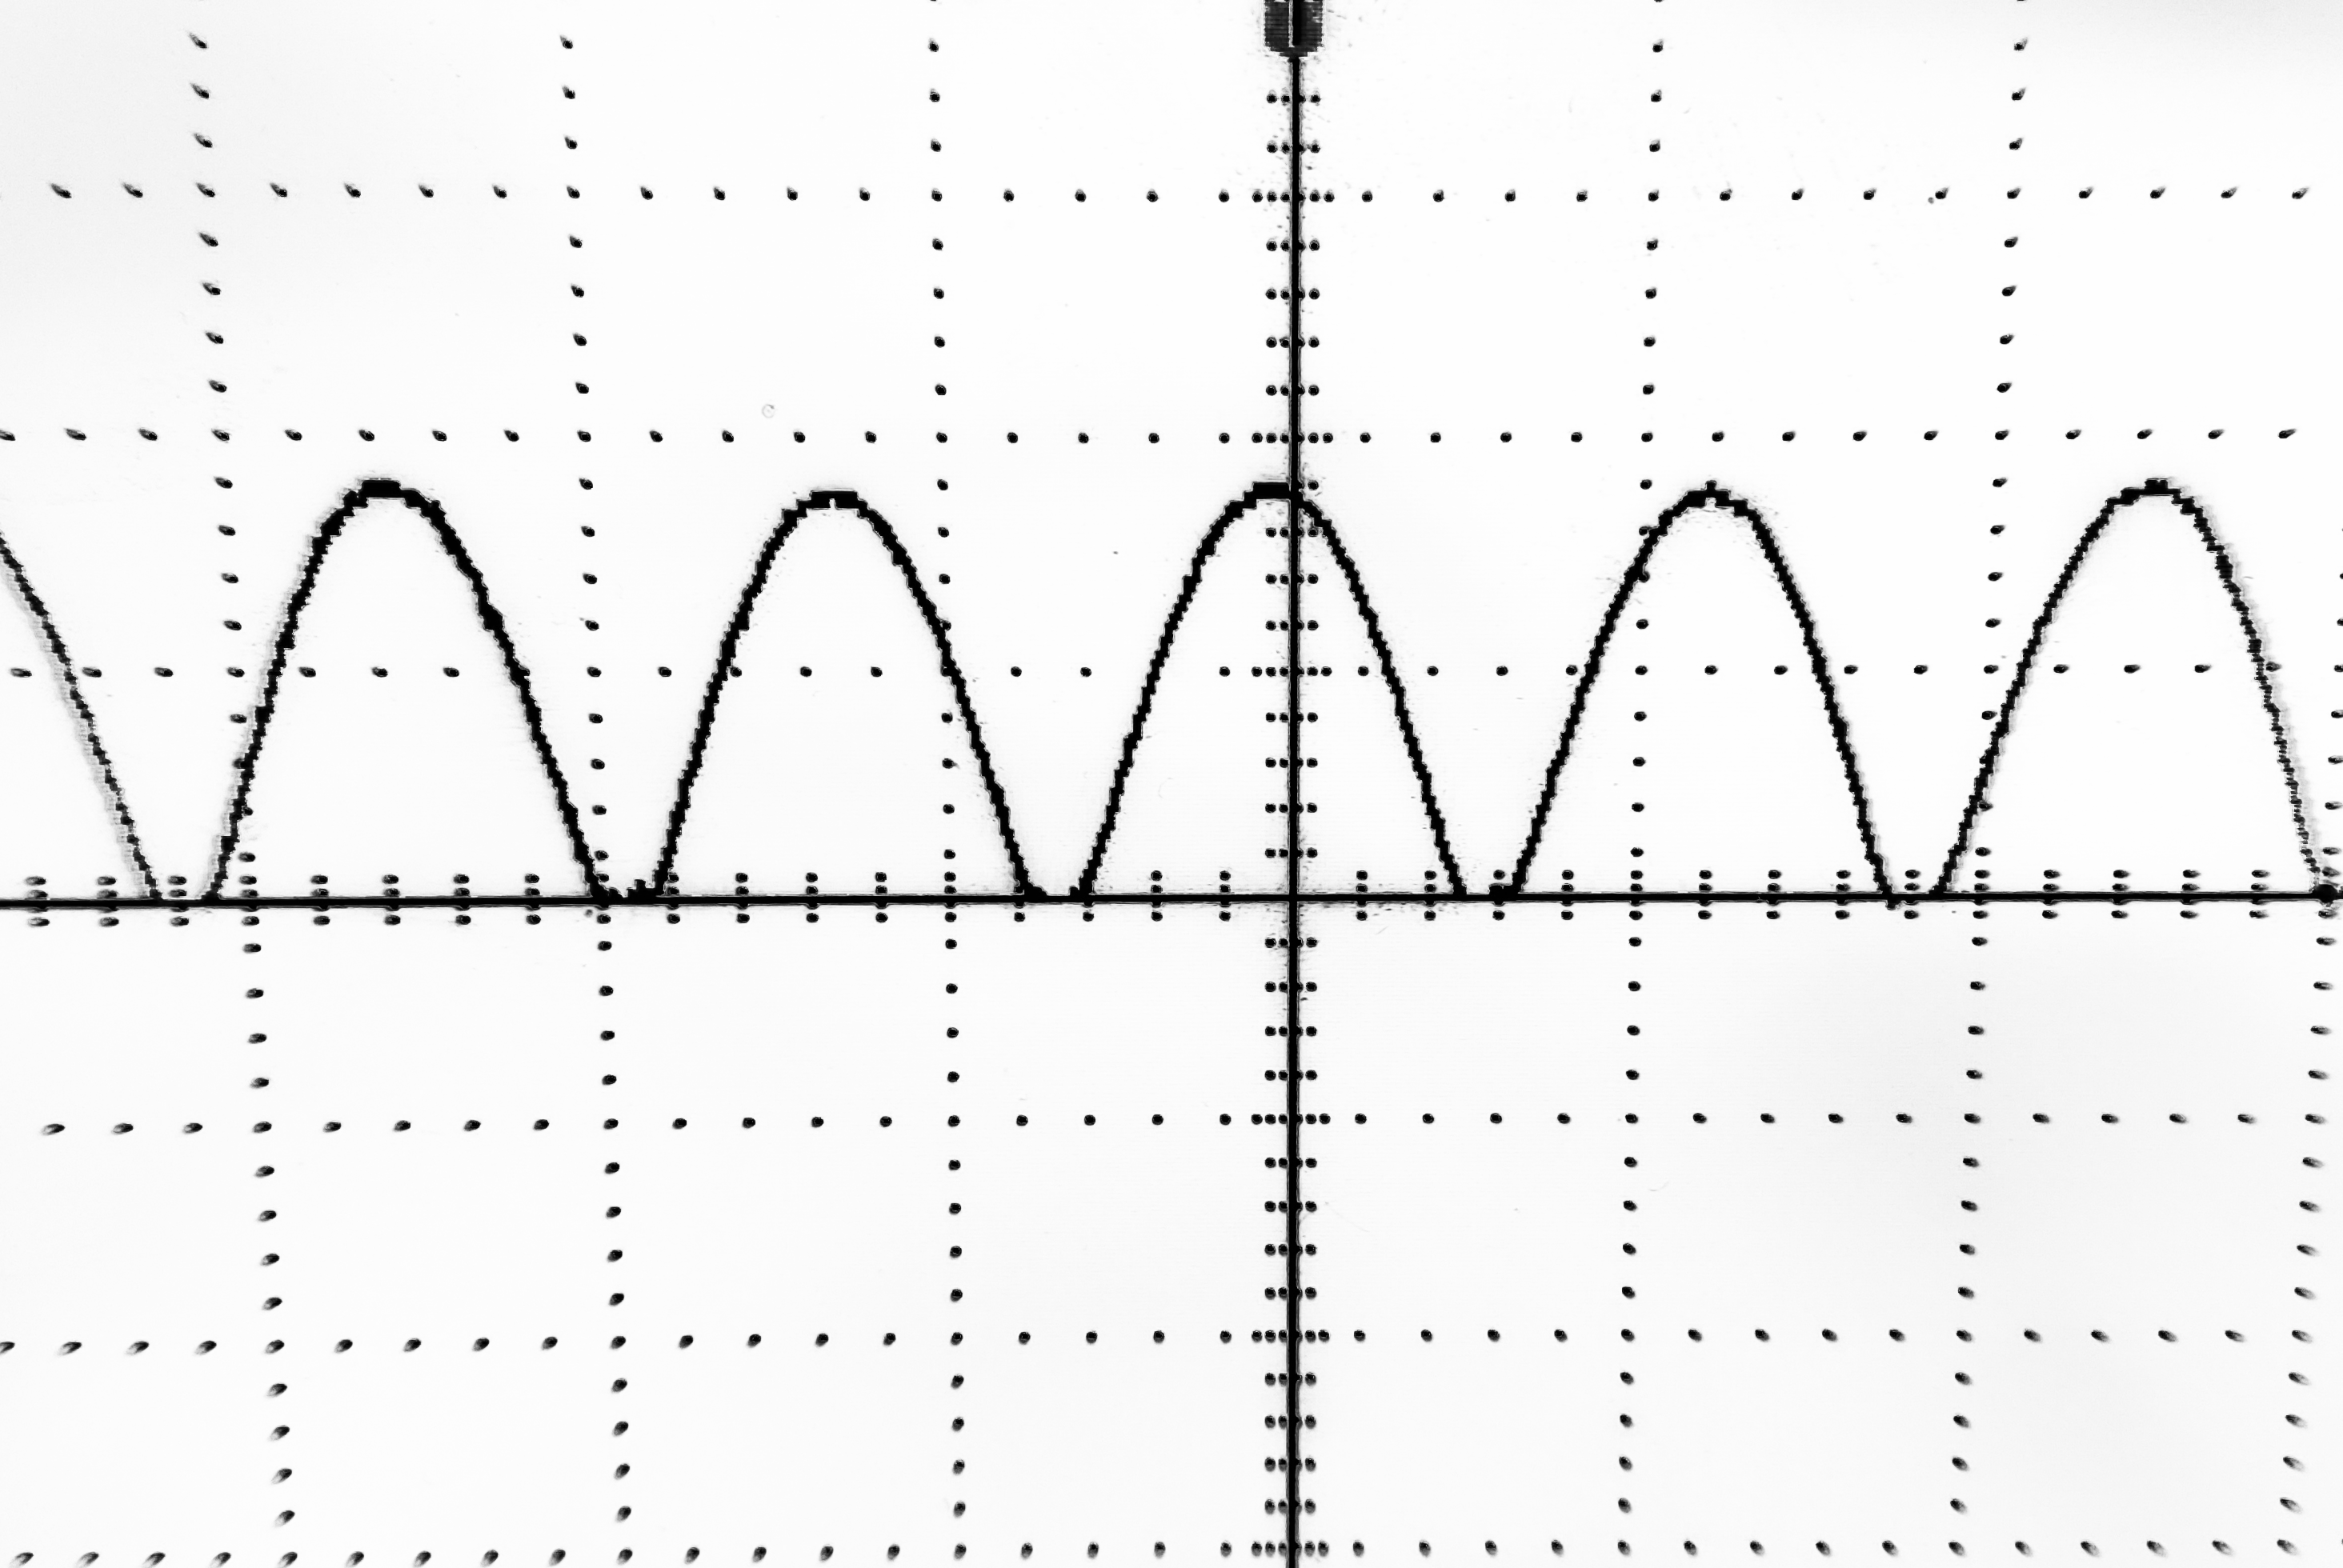
\includegraphics[scale=0.07]{figures/qbzl.png}
        \caption{全波整流波形图}
    \end{minipage}
\end{figure*}
\begin{figure*}[h]
    \centering
    \begin{minipage}[t]{0.48\textwidth}
        \centering
        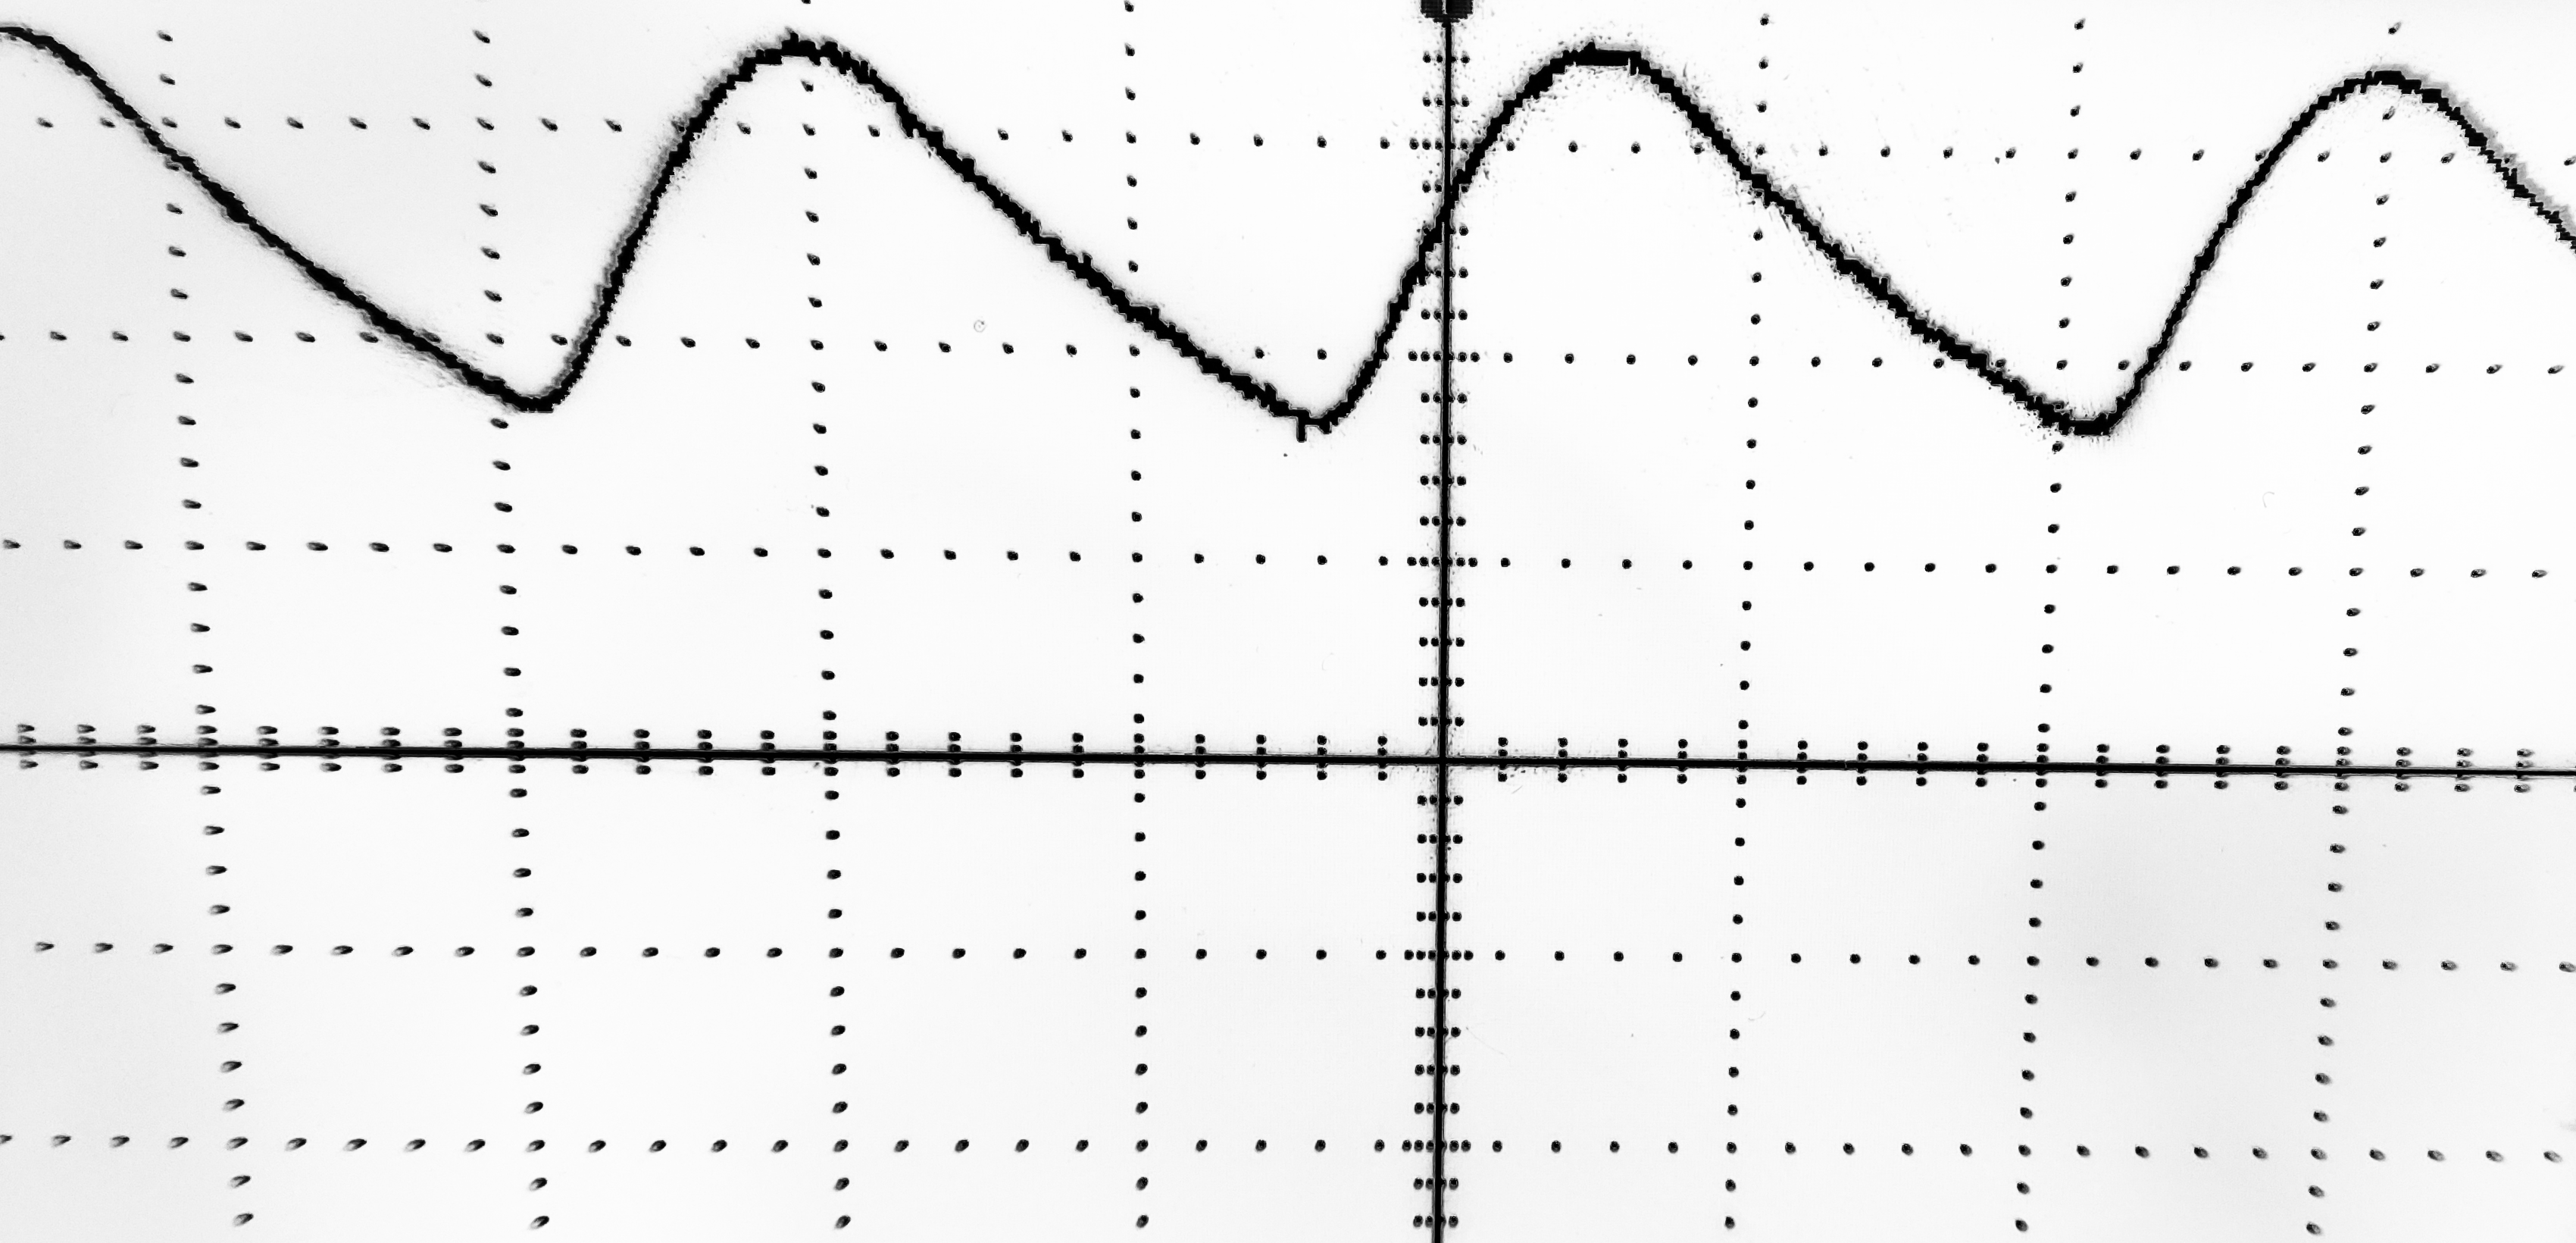
\includegraphics[scale=0.065]{figures/dr1.png}
        \caption{单电容滤波波形图}
    \end{minipage}
    \begin{minipage}[t]{0.48\textwidth}
        \centering
        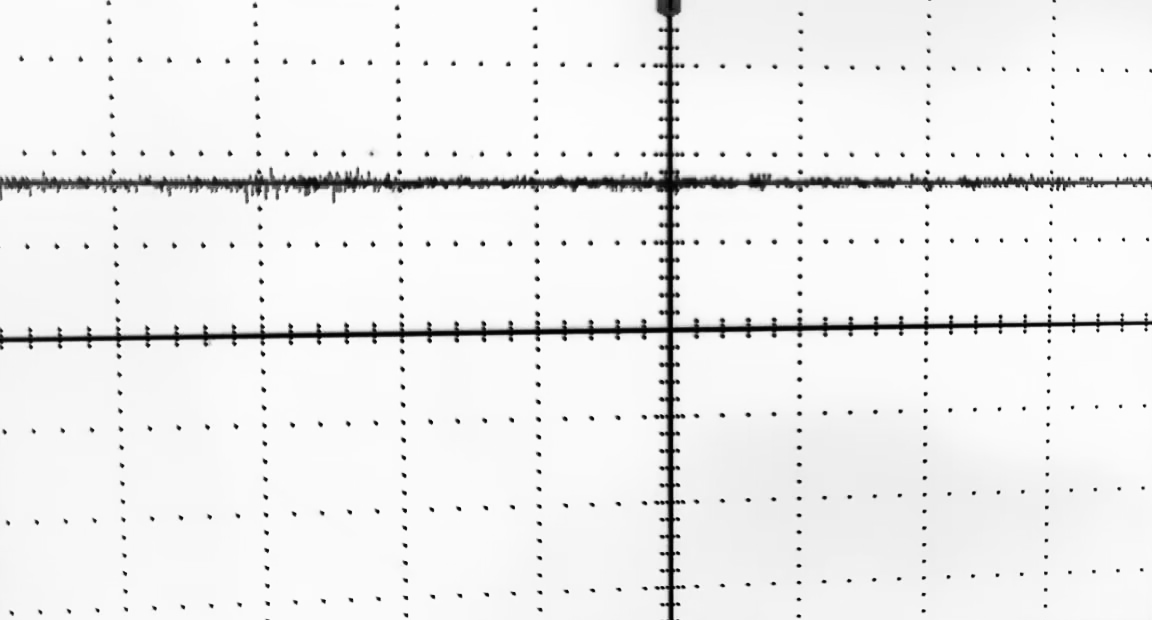
\includegraphics[scale=0.18]{figures/pi.png}
        \caption{$\pi$型RC滤波波形图}
    \end{minipage}
\end{figure*}

\begin{table}[htbp]
    \centering
    \begin{tabular}{|l|l|l|}
        \hline
             & 单电容滤波        & pi型RC滤波 \bigstrut \\
        \hline
        直流电压 DCV& \SI{2.58}{V} & \SI{1.60}{V}      \\
        \hline
        交流电压 ACV& \SI{575}{mV} & \SI{8.22}{mV}     \\
        \hline
        波纹系数 $K_u$ & 22.3\%       & 0.514\%           \\
        \hline
    \end{tabular}
\end{table}%

\subsection*{提升实验}
单电容滤波(\SI{10}{\mu F})的电压和波形图如下。

直流电压:\SI{2.93}{V} 交流电压: \SI{27.7}{mV}  波纹系数: 0.845\%
\begin{figure*}[htbp]
    
    \centering
    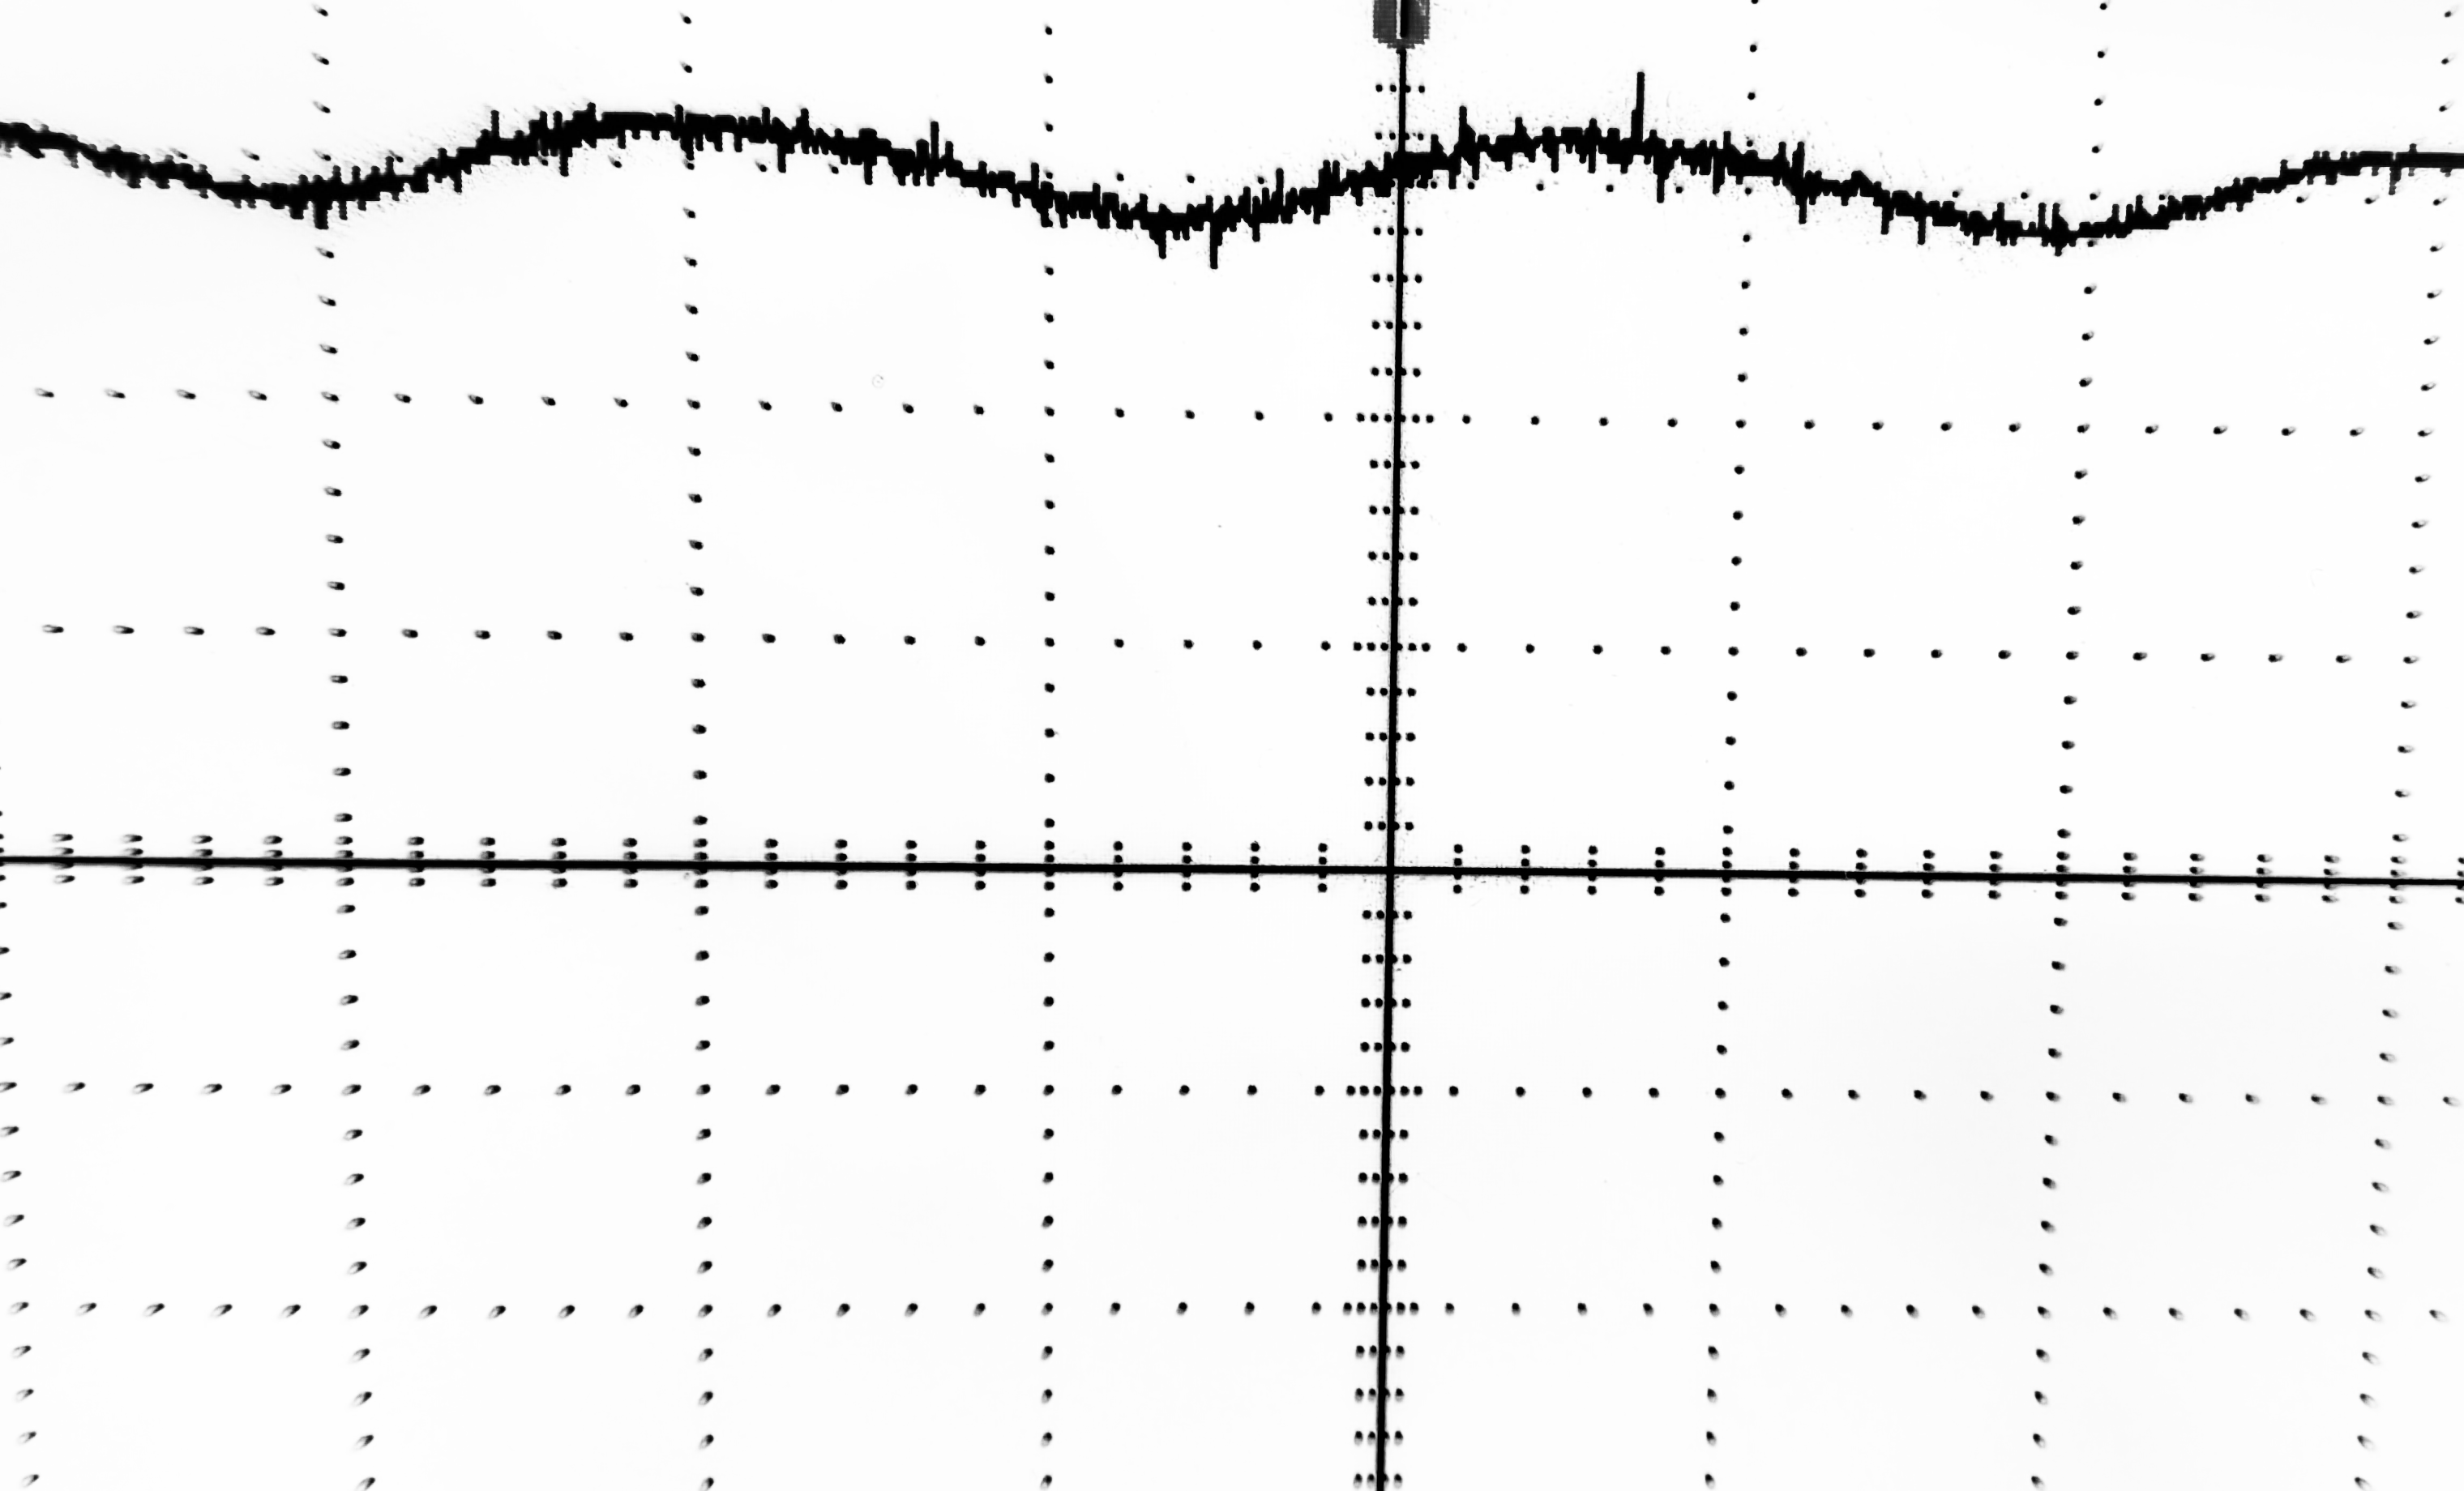
\includegraphics[scale=0.065]{figures/dr10.png}
    \caption{单电容滤波(\SI{10}{\mu F})波形图}

\end{figure*}



\section*{思考题}
\begin{enumerate}
    \item 整流、滤波的主要目的是什么?

          整流的主要目的是将交流电变换为直流电;滤波的主要目的是把大脉动直流电处理成平滑的脉动小的直流
          电。

    \item  滤波电路中电容是否越大越好?请根据实验过程简述理由。

          滤波电路中电容不是越大越好,理由如下:
          \begin{enumerate}
              \item 电容容量的增大,会使电路体积变大,增加成本。
              \item 电容上存在寄生电感,电容放电回路会在某个频点上发生谐振。电容越大,谐振频率越低,电容能有效补偿电流的频率范围也越小。
          \end{enumerate}


\end{enumerate}


\end{document}